\section{Dipole radiation. Dyadic Green's function. The Purcell effect: classical approach}

\begin{otherlanguage}{russian}	
	\textcolor{red}{На лекциях часть с уравнениями Максвелла была прочитана в СГС, но считаю, что лучше написать это в СИ, так как большинство статей по этой теме и тот же Новотный --- в СИ.}
\end{otherlanguage}

\subsection{Dipole radiation and dyadic Green's function}

Consider a point dipole $\vec{d}_0$ which is located in point $\vec{r}_0$. The electric current is given by
\begin{equation}
	\vec{j} = \rho \vec{v} = \sum_i q_i \delta(\vec{r} - \vec{r}_i) \dot{\vec{r}}_i = \dot{\vec{d}}_0 \delta(\vec{r} - \vec{r}_0).
	\label{eq:dipole_current}
\end{equation}

Let us state a problem to find the dipole field in space. If one wants something which is connected with electromagnetism then he should write Maxwell equations. So we do (in SI units)
\begin{numcases}{}
	\Rot \vec{E} = -  \parder{\vec{B}}{t},
	\label{eq:M1_j} \\
	\Rot \vec{H} = \parder{\vec{D}}{t} + \vec{j},
	\label{eq:M2_j} \\
	\Div \vec{D} = \rho,
	\label{eq:M3_j} \\
	\Div \vec{B} = 0.
	\label{eq:M4_j}
\end{numcases}
After applying the Fourier transform over time (in fact just $\partial_t \to - i \omega$) and using $\vec{D} = \varepsilon \varepsilon_0 \vec{E}$ and $\vec{B} = \mu \mu_0 \vec{H}$  we obtain
\begin{equation}
	\Rot \Rot \vec{E}  - \mu \mu_0 \varepsilon \varepsilon_0 \omega^2 \vec{E} =  i \mu \mu_0 \omega \vec{j}
\end{equation}
introducing $k = \dfrac{\omega}{c} \sqrt{\varepsilon \mu}$ we get
\begin{equation}
	\Rot \Rot \vec{E} - k^2 \vec{E} = \frac{k^2}{\varepsilon \varepsilon_0} \vec{d}_0 \delta(\vec{r} - \vec{r}_0).
	\label{eq:grrr}
\end{equation}
Here we have an inhomogeneous differential equation with a $\delta$--function on the rhs of the equation. Solution of such equation is a Green's function $\hat{\vec{G}}(\vec{r}, \vec{r}_0)$. As \eqref{eq:grrr} is in fact three equation then Green's function for a electromagnetic fields is a tensor or a so--called \textit{dyadic Green's function}. This fact is represent by writing a "hat" over $G$.
 
\subsubsection{Green's function. General information}

A Green's function, $G(x,s)$, of a linear differential operator $\hat{L}$ acting on distributions over a subset of the Euclidean space, at a point s, is any solution of
\begin{equation}
	\hat{L} G(x, s) = \delta(x - s).
\end{equation}
The knowledge of $G(x,s)$ allows us to write the solution in a straight forward way for any rhs part. In other words
\begin{equation}
	\hat{L} u(x) = f(x) \quad \to \quad u(x) = \int ds G(x,s) f(s).
\end{equation}

In our particular case, if we know the radiation of a dipole, we can calculate radiation for any complex current $\vec{j}(\vec{r})$.

\begin{testexample}[Field from an arbitrary current]
	\begin{equation}
		\vec{E}(\vec{r}) = i \begin{pmatrix}
			\dfrac{4 \pi}{c}  \\ \\
			\dfrac{1}{c \varepsilon_0}
		\end{pmatrix} k \int d^3r' \hat{\vec{G}}(\vec{r}, \vec{r}') \vec{j}(\vec{r}'), \qquad \text{units: }\begin{pmatrix}
		\text{sgs}  \\ \\
		\text{SI}
		\end{pmatrix}
		\label{eq:E_from_G}
	\end{equation}
	\textit{Remark:} $\hat{\vec{G}} \vec{j} = \vec{e}_i \hat{G}_{ik} j_k$, where $\vec{e}_i$ --- a unit vector.
\end{testexample}

\subsubsection{Derivation of the Green's function for Maxwell equations}

As we understand how it is convenient and important, let us find the explicit form for $\hat{\vec{G}}$. The general definition of the dyadic Green’s function for the electric field is
\begin{equation}
	\Rot \Rot \hat{\vec{G}}(\vec{r}, \vec{r}_0) - k^2 \hat{\vec{G}}(\vec{r}, \vec{r}_0) = \hat{\vec{I}} \delta(\vec{r} - \vec{r}_0).
\end{equation}
If we know $\hat{\vec{G}}$, then we know $\vec{E}$ from \eqref{eq:E_from_G}. On the other hand we know that
\begin{equation}
	\vec{E} = - \nabla \varphi - \parder{\vec{A}}{t}.
	\label{eq:elll}
\end{equation}
If we use electromagnetic potential $\vec{A}$ then we can choose any gauge for our convenience. Let us take the Lorenz gauge
\begin{equation}
	\Div \vec{A} + \frac{1}{c} \parder{\varphi}{t} = 0 \quad \to \quad \nabla \varphi = \frac{c}{i \omega} \nabla \Div \vec{A}.
\end{equation}
It means that $\varphi$ and $\vec{A}$ obeys
\begin{numcases}{\label{eq:gelm}}
	\Delta \vec{A} + k^2 \vec{A} = - \mu \mu_0 \vec{j}, \\
	\Delta \varphi + k^2 \varphi = - \frac{\rho}{\varepsilon \varepsilon_0}.	
\end{numcases}
As we can see \eqref{eq:gelm} ---inhomogeneous Helmholtz equations. The Green's function is known (careful derivation is too long and may take away from the main point):
\begin{equation}
	G_0(\vec{r}, \vec{r}_0) = \frac{e^{ikR}}{4\pi R}, \qquad R = \left| \vec{r} - \vec{r}_0 \right|.
\end{equation}
It means that we can write the solution of \eqref{eq:gelm} as
\begin{numcases}{\label{eq:solll}}
	\vec{A}(\vec{r}) = \mu \mu_0 \int d^3 r' G_0(\vec{r}, \vec{r}') \hat{\vec{I}} \vec{j}(\vec{r}'), \\
	\varphi(\vec{r}) = \frac{1}{\varepsilon \varepsilon_0} \int d^3r' G_0(\vec{r}, \vec{r}') \rho(\vec{r}'),
\end{numcases}
where $\hat{\vec{I}}_{ik} = \delta_{ik}$ --- a unit tensor. To get the final answer for $\hat{\vec{G}}$ we substitute \eqref{eq:solll} in \eqref{eq:elll} and compare the result with \eqref{eq:E_from_G}. Substitution gives
\begin{equation}
	\vec{E}(\vec{r}) = i \omega \mu \mu_0 \int d^3 r' \underbrace{\left[ G_0(\vec{r}, \vec{r}') \hat{\vec{I}} + \frac{1}{k^2} \nabla \Div G_0(\vec{r}, \vec{r}') \hat{\vec{I}} \right]}_{\hookrightarrow \myeq \hat{\vec{G}}(\vec{r}, \vec{r}')} \vec{j}(\vec{r}')
\end{equation}
or
\begin{equation}
	\hat{\vec{G}}(\vec{r}, \vec{r}_0) = \left( \hat{\vec{I}} + \frac{1}{k^2} \nabla \otimes \nabla \right) G_0(\vec{r}, \vec{r}_0),
	\label{eq:ggGGGgg}
\end{equation}
where $(\nabla \otimes \nabla)_{\alpha \beta} = \partial_{\alpha} \partial_{\beta}$, $\alpha, \beta = x,y,z$ --- a tensor product of $\nabla$.
 
\begin{testexample}[Field of a point dipole in vacuum]
	Let us assume a monochromic dipole, so from \eqref{eq:dipole_current} we obtain
	\begin{equation}
		\vec{j} = -i\omega \vec{d}_0 \delta(\vec{r} - \vec{r}_0).
		\label{eq:dipole_curr}
	\end{equation}
	Substitution to \eqref{eq:E_from_G} gives
	\begin{equation}
		\vec{E}(\vec{r}) = i \frac{1}{c \varepsilon_0}k (-i\omega) \int d^3 r' \hat{\vec{G}}(\vec{r}, \vec{r}') \vec{d}_0 \delta(\vec{r} - \vec{r}_0) = \frac{k^2}{\varepsilon_0} \hat{\vec{G}}(\vec{r}, \vec{r}_0) \vec{d}_0
		\label{eq:dipole_field}
	\end{equation}
	or
	\begin{equation}
		E_{\alpha}(\vec{r}) = \begin{pmatrix}
		4\pi  \\ \\
		\dfrac{1}{\varepsilon_0}
		\end{pmatrix} k^2  \hat{G}_{\alpha \beta}(\vec{r}, \vec{r}_0) d_{0 \beta} \qquad \text{units: }\begin{pmatrix}
		\text{sgs}  \\ \\
		\text{SI}
		\end{pmatrix}.
	\end{equation}
	\textit{Remark:} interesting to notice that is $\vec{d}_0 = (d_0,0,0)$ then the first column of $\hat{\vec{G}}$ shows a field which induces a dipole $Ox$-directed.
\end{testexample}

\subsubsection{Near-, intermediate- and far-field parts of Green's function}

Sometimes it is convenient to write  \eqref{eq:ggGGGgg} in different form:
\begin{equation}
	\hat{\vec{G}} (\vec{r}, \vec{r}_0) \overset{\vec{R} = \vec{r} - \vec{r}_0}{=} \hat{\vec{G}}(\vec{R}) = \frac{e^{ikR}}{4\pi R} \left[  \left( 1 + \frac{ikR - 1}{k^2R^2} \right) \hat{\vec{I}} + \frac{3 - 3ikR - k^2R^2}{k^2R^2} \frac{\vec{R}\otimes\vec{R}}{R^2} \right],
\end{equation}
which can be divided for summands with different powers of $kR$ as
\begin{equation}
	\hat{\vec{G}}(\vec{R}) = \hat{\vec{G}}_{NF} + \hat{\vec{G}}_{IF} + \hat{\vec{G}}_{FF},
	\label{eq:GGG}
\end{equation}
where
\begin{equation*}
	\begin{matrix}
		(\text{electrostatics}) & \hat{\vec{G}}_{NF} &=& \frac{e^{ikR}}{4\pi R} \frac{1}{k^2R^2} \left( 3 \frac{\vec{R}\otimes\vec{R}}{R^2} - \hat{\vec{I}} \right), & kR \ll 1 \\ \\
		& \hat{\vec{G}}_{IF} &=& \frac{e^{ikR}}{4\pi R} \frac{i}{kR}  \left( \hat{\vec{I}} - 3\frac{\vec{R}\otimes\vec{R}}{R^2} \right), & kR \sim 1 \\ \\
		(\text{electrodynamics})& \hat{\vec{G}}_{FF} &=& \frac{e^{ikR}}{4\pi R}  \left( \hat{\vec{I}} - \frac{\vec{R}\otimes\vec{R}}{R^2} \right), & kR \gg 1
	\end{matrix}
\end{equation*}
The simplified radiation spectrum and its connection with \eqref{eq:GGG} is shown in fig. \ref{fig:radiation1}.

\begin{figure}
	\centering
	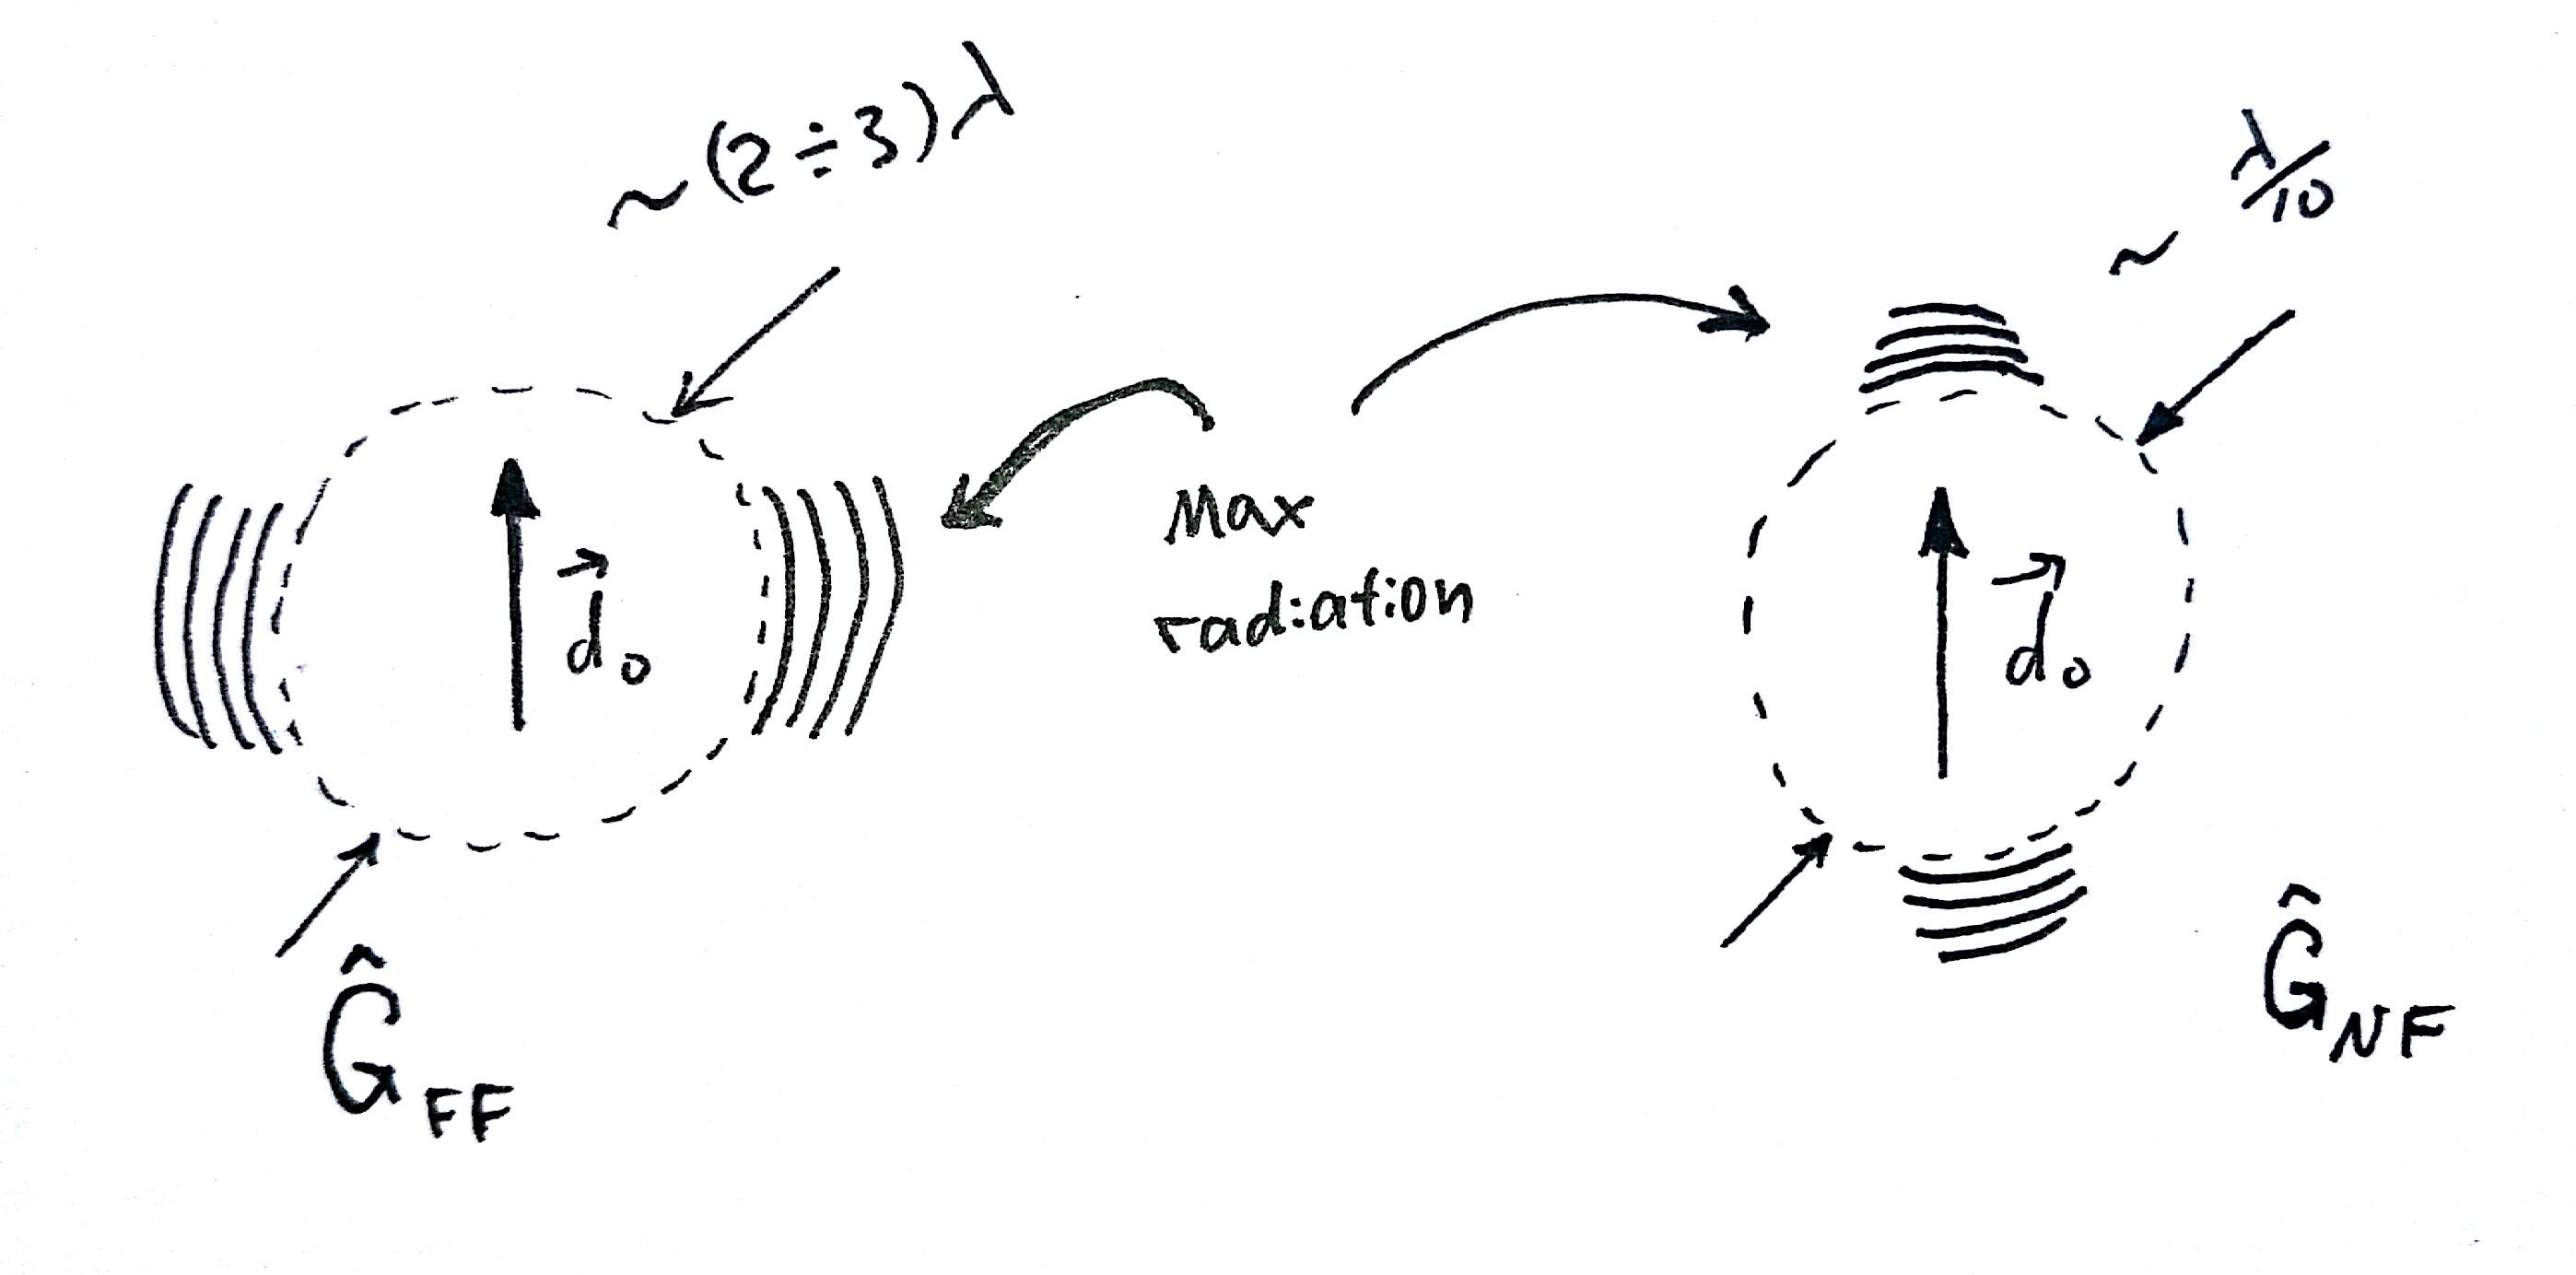
\includegraphics[width=0.6\linewidth]{fig/L8/radiation_1}
	\caption{Intuitive picture of positioning of maximum radiation of a dipole}
	\label{fig:radiation1}
\end{figure}


\subsection{Spontaneous relaxation and local density-of-state (IN A MIXED UNITS)}

\subsubsection{An expression for spontaneous decay}

Consider an excited atom which interacts with vacuum (fig. \ref{fig:relaxation}).	Relaxation may accrue to different channels which are related to a singe photon in different modes.

\begin{figure}
	\centering
	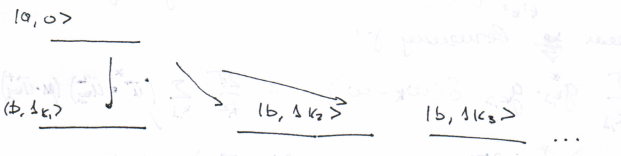
\includegraphics[width=0.7\linewidth]{fig/L8/relaxation}
	\caption{Transition from an initial state $\ket{a,0}$ to a set if final states $\ket{b, 1_{\left\{ \kv \right\}}}$. All the final states have the same energy. The states are products of atomic states and single--photon states.}
	\label{fig:relaxation}
\end{figure}

According to Fermi's Golden Rule the transition speed $\gamma$ is given by
\begin{equation}
	\gamma = \frac{2\pi}{\hbar^2} \sum_{f} \left| \bra{f} \hat{V} \ket{i} \right|^2 \delta(\omega_i - \omega_f),	\qquad \left[\gamma\right] = \left[\frac{1}{\text{time}}\right],
\end{equation}
where $\ket{f} =\ket{b, 1_{\left\{ \kv \right\}}}$ and $\ket{i} = \ket{a,0}$. In order to find it we need to calculate the matrix element. As we had above, perturbation operator is given by
\begin{equation}
	\hat{V} = \hbar \sum_{\kv, \lambda} g_{\kv, \lambda} \hat{\sigma}_+ \hat{a}_{\kv, \lambda} + \text{h.c.}
\end{equation}
and field operator 
\begin{equation}
	\hat{\vec{E}} = \sum_{\kv, \lambda} \varepsilon_{\kv} e^{i \vec{k} \vec{r} - i \omega_{\kv}t} \vec{e}_{\vec{r}, \lambda} \hat{a}_{\kv, \lambda} + \text{h.c.} = \hat{\vec{E}}^+ + \hat{\vec{E}}^-, \qquad \varepsilon_{\kv} = \sqrt{\frac{2 \pi \hbar \omega_{\kv}}{V}},
\end{equation}
which is convenient to rewrite as 
\begin{equation}
	\hat{\vec{E}}^+ = \sum_{\kv, \lambda} \varepsilon_{\kv} e^{i\vec{k} \vec{r}} \vec{e}_{\kv , \lambda} \hat{a}_{\kv, \lambda} e^{-i\omega_{\kv} t} = \sum_{\kv, \lambda} \vec{u}_{\kv, \lambda}^+(\vec{r}) \hat{a}_{\kv, \lambda} e^{-i\omega_{\kv}},
\end{equation}
where $\vec{u}_{\kv}^+(\vec{r})$ --- a vector of a mode which contains all the information about the system which is quantized. Omitting the computational details we have
\begin{equation}
	\left| \bra{f} \hat{V} \ket{i} \right|^2 =  \hbar^2 \left| g_{\kv, \lambda} \right|^2 ,
\end{equation}
so
\begin{equation}
	\gamma = \frac{2\pi}{\hbar^2} \sum_{\kv, \lambda} \hbar^2 \left| g_{\kv, \lambda} \right|^2 \delta(\omega_{\kv} - \omega).
\end{equation}
Using the fact that $g_{\kv, \lambda} = - \frac{\vec{d} \cdot \vec{u}^+_{\kv, \lambda}}{\hbar}$ we have
\begin{multline}
	\gamma = \frac{2\pi}{\hbar^2} \sum_{\kv, \lambda} \left( \vec{d} \cdot \vec{u}_{\kv, \lambda}^+ \right)^* \left( \vec{d} \cdot \vec{u}_{\kv, \lambda}^+ \right) \delta(\omega_{\kv} - \omega) = \frac{2\pi}{\hbar^2} \sum_{\kv, \lambda} \vec{d}^* \left(\vec{u}_{\kv, \lambda}^- \otimes  \vec{u}_{\kv, \lambda}^+ \right) \vec{d} \delta(\omega_{\kv} - \omega)= \\ =
	\Bigg/ \vec{u}^+_{\vec{k}, \lambda} = \varepsilon_{\kv} e^{i \vec{k} \vec{r}} \vec{e}_{\kv \lambda} =  \sqrt{2\pi \hbar \omega_{\kv}} \cdot \frac{1}{\sqrt{V}} \vec{e}_{\kv \lambda} e^{i \kv \vec{r}} \myeq \sqrt{2\pi \hbar \omega_{\kv}} \vec{u}^{0+}_{\kv \lambda} \Bigg/ =  \\ = \frac{2\pi}{\hbar^2} \hbar \omega 2 \pi  |\vec{d}|^2 \sum_{\kv, \lambda} \vec{n}^* \left( \vec{u}^{0+}_{\kv \lambda} \otimes \vec{u}^{0-}_{\kv \lambda} \right) \vec{n} \delta (\omega_{\kv} - \omega) , \qquad \vec{d} = |\vec{d}| \vec{n}.
\end{multline}
\begin{otherlanguage}{russian}	
	\textcolor{red}{Не понятно как здесь получилось вынести $\omega_{\kv}$ из под суммы превратить её в $\omega$. Что на лекциях так было, что у вас в конспекте.}
\end{otherlanguage}
Now we introduce the \textit{local density-of-state} which contains all the information about the system
\begin{equation}
	\rho_{\vec{d}} (\vec{r}, \omega) \myeq 3 \sum_{\kv, \lambda} \vec{n}^* \left( \vec{u}^{0+}_{\kv \lambda} \otimes \vec{u}^{0-}_{\kv \lambda} \right) \vec{n} \delta (\omega_{\kv} - \omega),
\end{equation}
then
\begin{equation}
	\boxed{	\gamma  = \frac{4 \pi^2 \omega_0}{3 \hbar} |\vec{d}|^2 \rho_{\vec{d}}, \qquad |\vec{d}|^2 = \left|  \bra{a} e \vec{r} \ket{b} \right|^2. }
	\label{eq:gamma_start}
\end{equation}

\subsubsection{Spontaneous decay and Green's dyadics}

After that need apply a Hilbert–Schmidt formula 
\begin{equation}
	\hat{\vec{G}} (\vec{r}, \vec{r}_0, \omega) \sum_{\kv, \lambda} \frac{\left( \vec{u}^{0+}_{\kv \lambda} \otimes \vec{u}^{0-}_{\kv \lambda} \right)}{\frac{\omega_{\kv}^2}{c^2} - \frac{\omega^2}{c^2}}.
\end{equation}
Using Sokhotski formula
\begin{equation}
	\Im \left\{ \frac{1}{\omega_{\kv}^2 - \omega_{0}^2} \right\} = \frac{\pi}{2 \omega_{\kv}} \left( \delta(\omega_{\kv} - \omega_{0}) + \underbrace{\delta(\omega_{\kv} + \omega_{0})}_{\hookrightarrow=0,\ \omega_{\kv}>0}\right).
\end{equation}
Let us consider the imaginary part of the dyadic Green's function
\begin{equation}
	\Im \left\{ \hat{\vec{G}}(\vec{r}, \vec{r}_0, \omega) \right\} = \frac{\pi c^2}{2 \omega} \sum_{\kv, \lambda} \left( \vec{u}^{0+}_{\kv \lambda} (\vec{r}) \otimes \vec{u}^{0-}_{\kv \lambda} (\vec{r}_0) \right) \delta (\omega - \omega_{\kv}),
\end{equation} 
then the local density-of-state
\begin{equation}
	\rho_{\vec{d}} (\vec{r}_0, \omega) = \frac{6 \omega}{\pi c^2} \left( \vec{n}^* \cdot \Im \left\{ \hat{\vec{G}} (\vec{r}_0, \vec{r}_0, \omega) \right\} \cdot \vec{n} \right).
\end{equation}
The main thing to notice is
\begin{equation}
	\boxed{	\gamma \sim \rho_{\vec{d}} (\vec{r}_0, \omega) \sim \Im \left\{ \hat{\vec{G}} (\vec{r}_0, \vec{r}_0, \omega) \right\}.}
\end{equation}

Now let us calculate the spectral density of state
\begin{equation}
	D(\omega) = \int d^3 r_0 \rho_{\vec{d}} (\vec{r}_0, \omega),
\end{equation}
then we find averaging over different orientations
\begin{equation}
	\langle \rho_{\vec{d}} \rangle_{\text{orientations}} = \frac{6 \omega}{\pi c^2} \frac{1}{3} \Im \left\{ \Tr \hat{\vec{G}} \right\} = \frac{\omega^2}{\pi^2 c^3},
\end{equation}
here we used
\begin{equation}
	\Im \left\{ \hat{G}_{\alpha \alpha} (\vec{r}_0, \vec{r}_0, \omega) \right\} = \frac{k}{6 \pi}, \qquad \alpha = x,y,z.
\end{equation}
\textit{Remark:} the real part has singularity
\begin{equation}
	\lim\limits_{\vec{r}\to \vec{r}_0}\Re \left\{ \hat{G}_{\alpha \alpha} (\vec{r}, \vec{r}_0, \omega) \right\}  = \infty,  \qquad \alpha = x,y,z.
\end{equation} 

Substitution to \eqref{eq:gamma_start} gives us
\begin{equation}
	\text{(vacuum)} \qquad \gamma_0 = \frac{4 |\vec{d}|^2 \omega^3}{3 \pi \hbar c^3}  \text{ [sgs]} = \frac{|\vec{d}|^2 \omega^3}{3 \hbar \varepsilon_0 \pi c^3} \text{ [SI]}.
\end{equation}
For medium with $n = \sqrt{\varepsilon_m}$ but \textit{with the same Green's function} we have
\begin{equation}
\text{(medium)} \qquad \gamma_0 = \frac{4 |\vec{d}|^2 \omega^3}{3 \pi \hbar c^3}n  \text{ [sgs]} = \frac{|\vec{d}|^2 \omega^3}{3 \hbar \varepsilon_0 \pi c^3}n \text{ [SI]}.
\end{equation}
\begin{otherlanguage}{russian}	
	\textcolor{red}{Оформить это в пример в разделе про фактор Парселла!} 
\end{otherlanguage}

\begin{otherlanguage}{russian}	
	\textcolor{red}{Надо тут все аккуратно с разномерносятми посмотреть, привести всё к СИ, либо всё в СГС.}
\end{otherlanguage}

\begin{otherlanguage}{russian}	
	\textcolor{red}{Тут ещё был пример про материалы, у которых $\varepsilon_x>0$, но $\varepsilon_y<0$ и какая-то глубокая мысль по этому поводу.}
\end{otherlanguage}

\subsection{The Purcell factor}

The Purcell factor is defined as 
\begin{equation}
	F_p \myeq \frac{\gamma}{\gamma_0} = \frac{\Im \left\{\vec{n} \hat{\vec{G}}_{\text{new}} \vec{n}\right\}}{\Im \left\{\vec{n} \hat{\vec{G}} \vec{n}\right\}} = 1 + \frac{\Im \left\{\vec{n} \hat{\vec{G}}_{\text{ext}} \vec{n}\right\}}{\Im \left\{\vec{n} \hat{\vec{G}} \vec{n}\right\}} = 1 + \frac{\Im \left\{\vec{n} \hat{\vec{G}}_{\text{ext}} \vec{n}\right\}}{k / 6\pi},
\end{equation}
where $\hat{\vec{G}}_{\text{new}} = \hat{\vec{G}} + \hat{\vec{G}}_{\text{ext}}$, $\gamma$ --- transition probability in a new media with its own $\hat{\vec{G}}_{\text{new}}$.

\begin{otherlanguage}{russian}	
	\textcolor{red}{Как получился переход $ \vec{n}^* \Im \left\{ \hat{\vec{G}}  \right\} \vec{n} \to \Im \left\{\vec{n} \hat{\vec{G}} \vec{n} \right\}$ ?} 
\end{otherlanguage}

Now let us take a look from the classical standpoint. Radiation power is given by the integral
\begin{equation}
	P = - \frac{1}{2} \Re \int d^3 r \vec{j}^* \vec{E},
\end{equation}
where dipole current and field is given by \eqref{eq:dipole_curr} and \eqref{eq:dipole_field} respectively. After substitution we obtain
\begin{multline}
	\text{(sgs):} \qquad P = \frac{\omega^2}{2} \Im \int d^3 r 4 \pi k^2 \vec{d}^* \hat{\vec{G}}(\vec{r}, \vec{r}_0, \omega) \vec{d} \delta(\vec{r} - \vec{r}_0) =\\= 2 \pi k^2 \omega |\vec{d}| \Im \left\{ \hat{\vec{G}} (\vec{r}_0, \vec{r}_0, \omega) \right\} = 2 \pi k^2 \omega |\vec{d}| \cdot \frac{k}{6 \pi}
\end{multline} 
and we've got the Rayleigh formula
\begin{equation}
	P = \frac{k^3 \omega |\vec{d}|^2}{3} \sim \omega^4.
\end{equation}

If a dipole is dieing  down then its energy
\begin{equation}
	W(t) = W(0) e^{- \gamma t}
\end{equation}
and radiation power
\begin{equation}
	P(t) = \frac{d}{dt} W(t) = - \gamma W(t).
\end{equation}
At time $t \approx 0$ we obtain
\begin{equation}
	\frac{P_{\text{medium}}(t)}{P_{\text{vacuum}}(t)} \approx \frac{\gamma}{\gamma_0} = F_p.
\end{equation}
We have the same result but only using the classical approach. But one needs to remember that the reason of radiation has a quantum nature.